% Digital Logic Report Template
% Created: 2020-01-10, John Miller

%==========================================================
%=========== Document Setup  ==============================

% Formatting defined by class file
\documentclass[11pt]{article}

% ---- Document formatting ----
\usepackage[margin=1in]{geometry}	% Narrower margins
\usepackage{booktabs}				% Nice formatting of tables
\usepackage{graphicx}				% Ability to include graphics

%\setlength\parindent{0pt}	% Do not indent first line of paragraphs 
\usepackage[parfill]{parskip}		% Line space b/w paragraphs
%	parfill option prevents last line of pgrph from being fully justified

% Parskip package adds too much space around titles, fix with this
\RequirePackage{titlesec}
\titlespacing\section{0pt}{8pt plus 4pt minus 2pt}{3pt plus 2pt minus 2pt}
\titlespacing\subsection{0pt}{4pt plus 4pt minus 2pt}{-2pt plus 2pt minus 2pt}
\titlespacing\subsubsection{0pt}{2pt plus 4pt minus 2pt}{-6pt plus 2pt minus 2pt}

% ---- Hyperlinks ----
\usepackage[colorlinks=true,urlcolor=blue]{hyperref}	% For URL's. Automatically links internal references.

% ---- Code listings ----
\usepackage{listings} 					% Nice code layout and inclusion
\usepackage[usenames,dvipsnames]{xcolor}	% Colors (needs to be defined before using colors)

% Define custom colors for listings
\definecolor{listinggray}{gray}{0.98}		% Listings background color
\definecolor{rulegray}{gray}{0.7}			% Listings rule/frame color

% Style for Verilog
\lstdefinestyle{Verilog}{
	language=Verilog,					% Verilog
	backgroundcolor=\color{listinggray},	% light gray background
	rulecolor=\color{blue}, 			% blue frame lines
	frame=tb,							% lines above & below
	linewidth=\columnwidth, 			% set line width
	basicstyle=\small\ttfamily,	% basic font style that is used for the code	
	breaklines=true, 					% allow breaking across columns/pages
	tabsize=3,							% set tab size
	commentstyle=\color{gray},	% comments in italic 
	stringstyle=\upshape,				% strings are printed in normal font
	showspaces=false,					% don't underscore spaces
}

% How to use: \Verilog[listing_options]{file}
\newcommand{\Verilog}[2][]{%
	\lstinputlisting[style=Verilog,#1]{#2}
}




%======================================================
%=========== Body  ====================================
\begin{document}

\title{ELC 2137 Lab 4: Subtractor}
\author{Jake Simmons and Haonan Jin }

\maketitle


\section*{Summary}

In this experiment we made a subtractor from a adder. First we made an adder by combining two full adders which is a two-bit adder. Then we added three XOR Gates, this was becasue we needed to invert two of our inputs to generate the 2's complement. The third XOR Gate inverted the carry out bit because Figure 3 shows that the carry out bit in our expected results was the opposite of what it should have been mathematically.


\section*{Q\&A}

\begin{enumerate}
	\item Why did we use two full adders instead of a half adder and a full adder?
	
		We used two full adders instead of a half adder and a full adder becasue if we used a half adder and full adder we would not get all three outputs. We would lose the S2 and Cout outputs.  

	\item How many input combinations would it take to exhaustively test the adder/subtractor?
	
		It would take 16 combinations to exhaustively test the adder/subtractor. 

	\item Why were the combinations given in the truth table chosen?
	
		The combinations given in the truth table were chosen to show that using the 2's complement in binary to subtract numbers does not always work.

	\item Do the results from your adder/subtractor match what you would expect from theory? Explain any discrepancies.
	
		The results from our adder/subtractor do not match what was expected from theory. This is becasue the actual adder/subtractor has 5 inputs while based on theory there are only four inputs. The 5th input is a carry in bit which when missing causes the carry out bit to be opposite in theory compared to the actual results. 

\end{enumerate}


\section*{Results}

\begin{center}
	\begin{figure}
		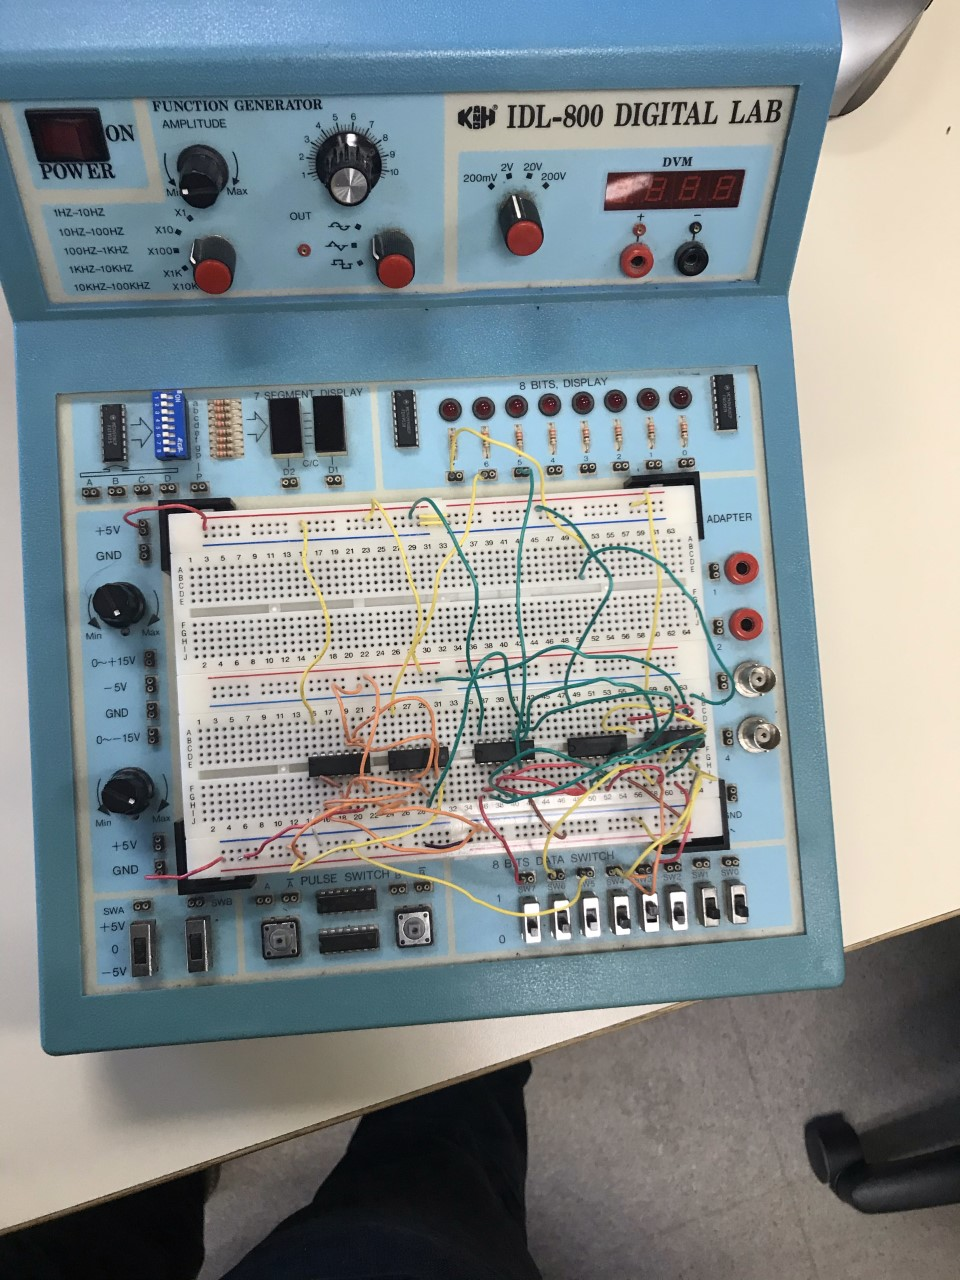
\includegraphics[width=1\textwidth]{thumbnail_Image.jpg}
		\caption{Picture of Assembled Circuit}
	\end{figure}
\end{center}

\begin{center}
	\begin{figure}
		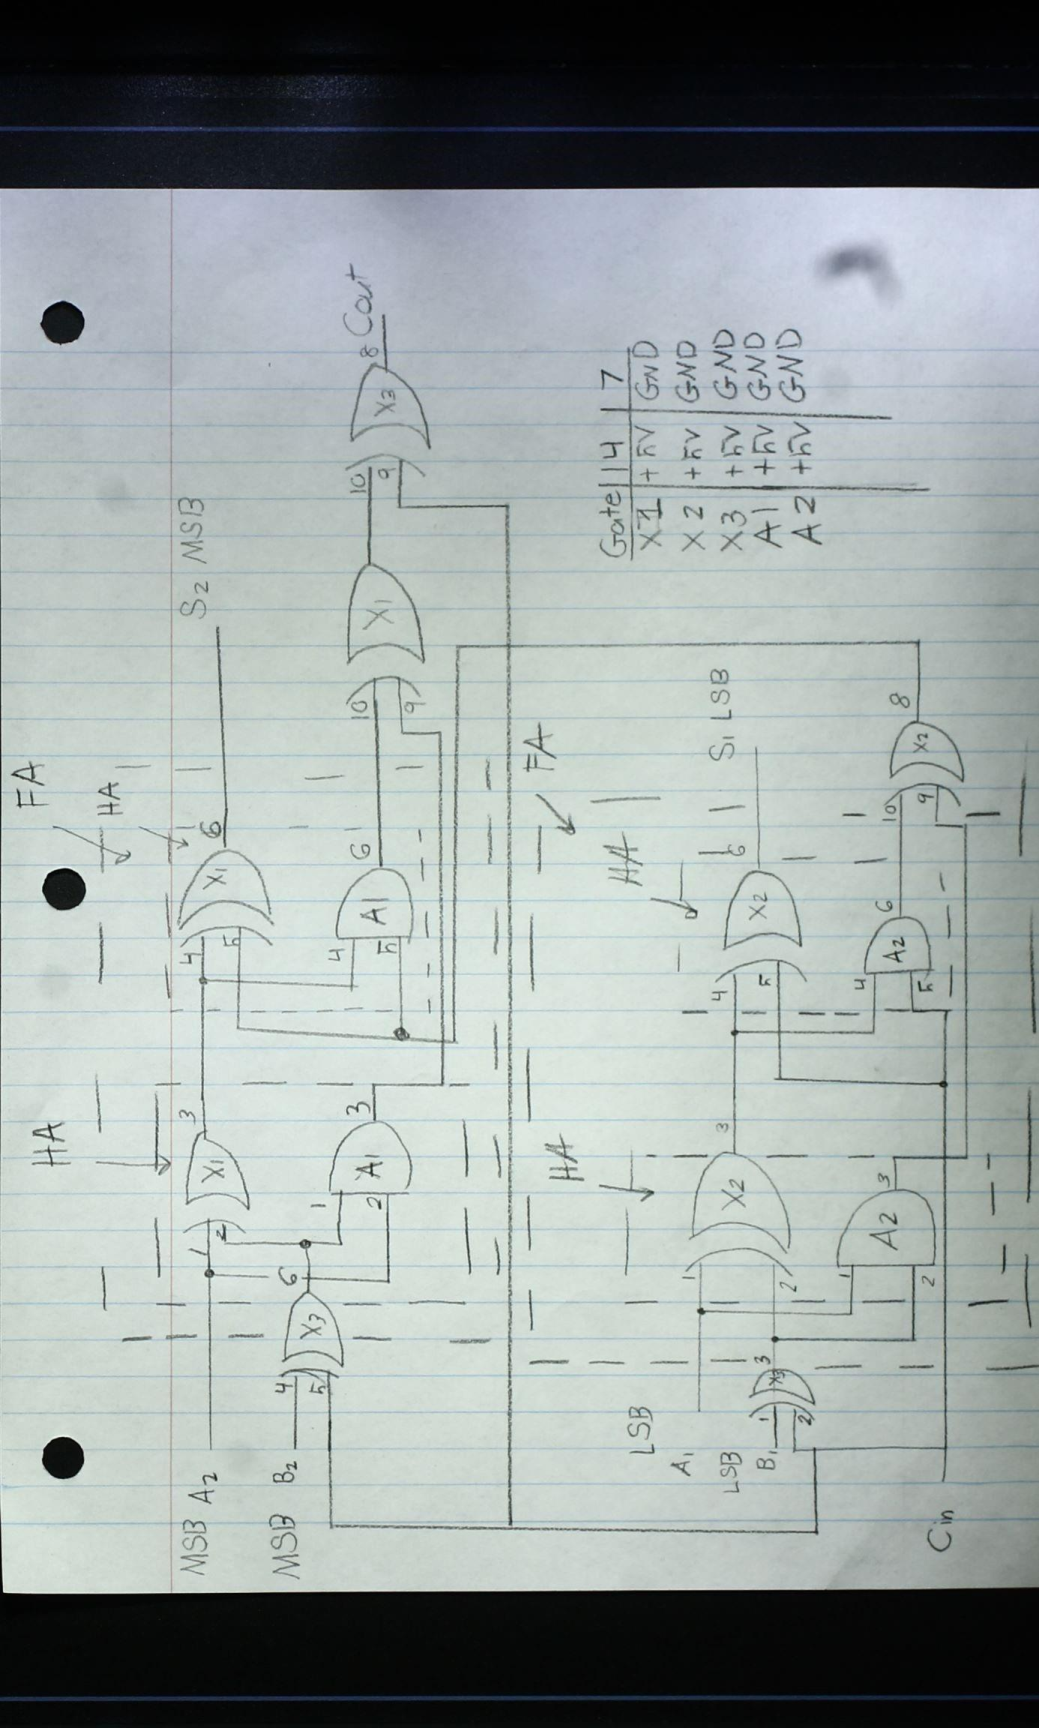
\includegraphics[width=.8\textwidth]{scanj.pdf}
		\caption{Two-Bit Adder/Subtractor Schematic}
	\end{figure}
\end{center}
\begin{center}
	\begin{figure}
		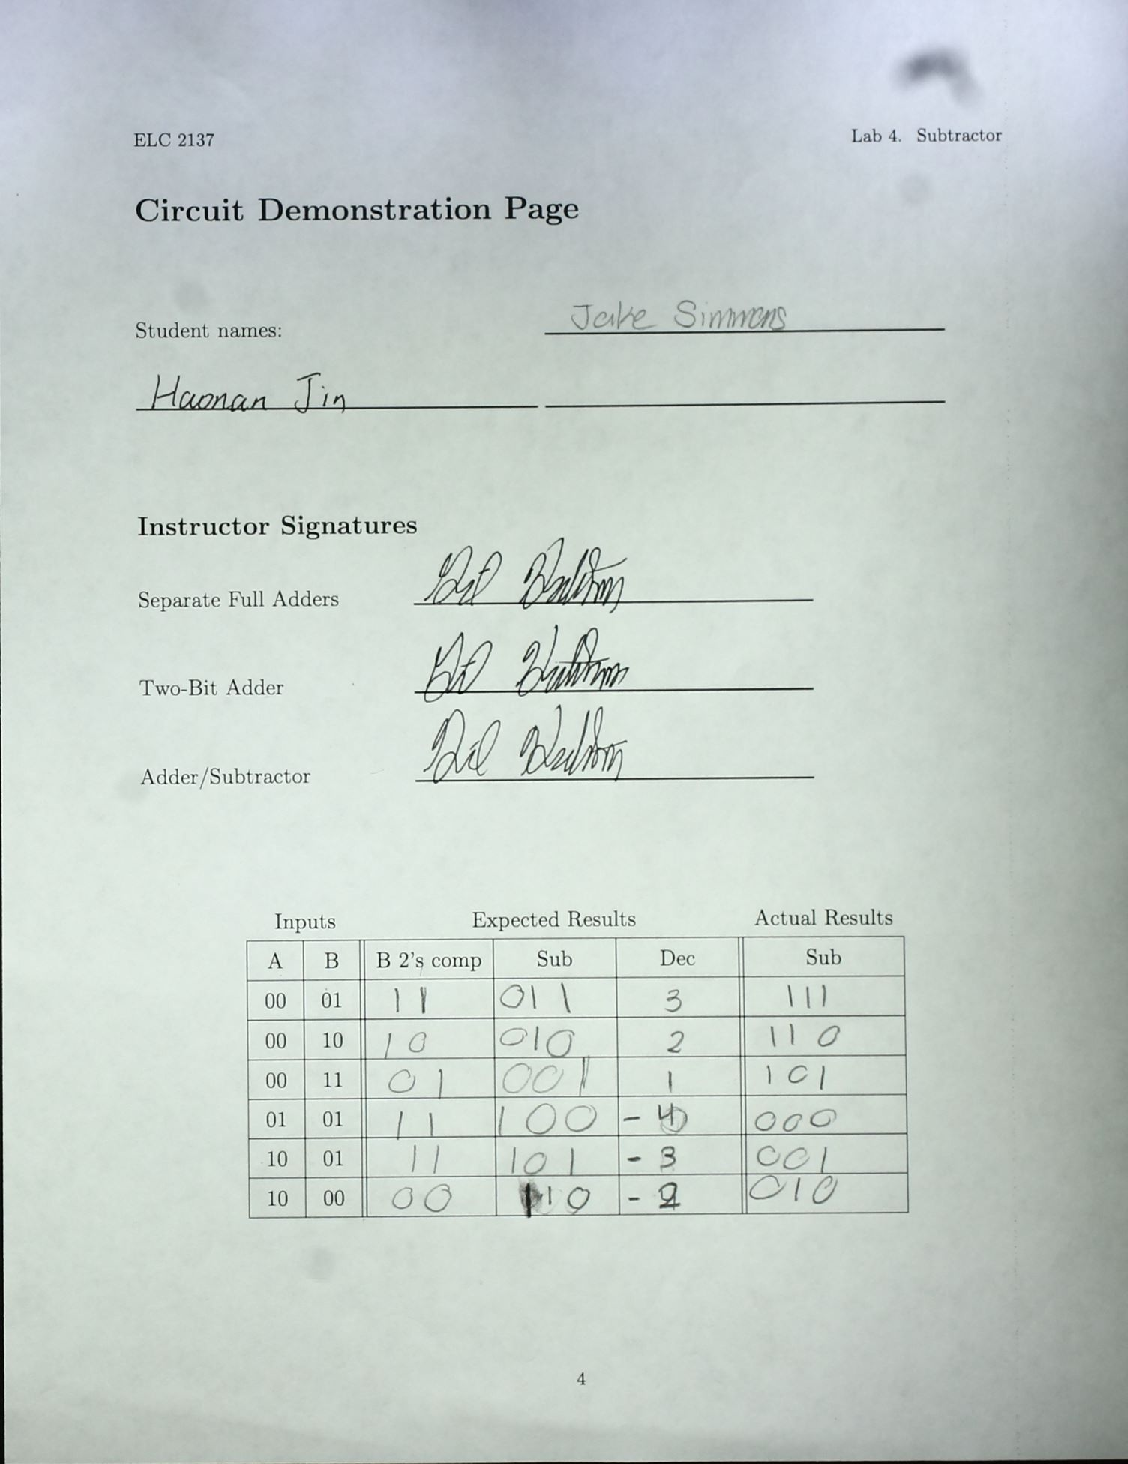
\includegraphics[width=1\textwidth]{KIC_Document.pdf}
		\caption{Circuit Demonstration Page}
	\end{figure}
\end{center}

\clearpage
\section*{Code}



\end{document}
